\documentclass[../notes.tex]{subfiles}

\pagestyle{main}
\renewcommand{\chaptermark}[1]{\markboth{\chaptername\ \thechapter\ (#1)}{}}
\setcounter{chapter}{8}

\begin{document}




\chapter{Rigid Body Motion}
\section{Introduction; Rotation About an Axis; Moments of Inertia}
\begin{itemize}
    \item \marginnote{11/3:}Announcements.
    \begin{itemize}
        \item We will now have \emph{seven} problem sets instead of \emph{eight}.
        \begin{itemize}
            \item Each problem set is now worth more (PSets still amount to 40\% of our grade).
            \item There will still be one makeup PSet at the end of the quarter.
        \end{itemize}
        \item PSet 5 is due next Friday.
    \end{itemize}
    \item Recap: Many-body motion.
    \begin{itemize}
        \item It's useful to introduce the center of mass coordinate, $\vec{R}=1/M\cdot\sum_\alpha m_\alpha\vec{r}_\alpha$, where $M=\sum_\alpha m_\alpha$.
        \item In the CM frame, $\vec{R}{\,}^*=0$ and $\vec{r}_\alpha=\vec{R}+\vec{r}_\alpha{}^*$.
        \begin{itemize}
            \item We also have $\vec{P}{\,}^*=0$, $T^*=\sum_\alpha m_\alpha(\dot{\vec{r}}_\alpha{}^*)^2/2$, and $\vec{J}{\,}^*=\sum_\alpha m_\alpha\vec{r}_\alpha{}^*\times\dot{\vec{r}}_\alpha{}^*$.
        \end{itemize}
        \item Then, going back into the lab frame, we have $\vec{P}=M\cdot\dot{\vec{R}}$, $T=M\dot{\vec{R}}^2/2+T^*$, and $\vec{J}=M\vec{R}\times\dot{\vec{R}}+\vec{J}{\,}^*$.
        \item One more note before we move onto rigid bodies: Suppose we're interested in the work, i.e., the rate of change of $T$ in the system.
        \begin{itemize}
            \item Recall that $m\ddot{\vec{r}}_\alpha=\sum_\beta\vec{F}_{\alpha\beta}+\vec{F}_\alpha$.
            \item Thus,
            \begin{equation*}
                \dot{T} = \sum_\alpha m_\alpha\dot{\vec{r}}_\alpha\cdot\ddot{\vec{r}}_\alpha
                = \sum_\alpha\sum_\beta\dot{\vec{r}}_\alpha\cdot\vec{F}_{\alpha\beta}+\sum_\alpha\dot{\vec{r}}_\alpha\cdot\vec{F}_\alpha
            \end{equation*}
            \item Note: Even letting $\vec{r}_{\alpha\beta}=\vec{r}_\alpha-\vec{r}_\beta$ and using $\vec{F}_{\alpha\beta}=-\vec{F}_{\beta\alpha}$, the left term above is often not equal to zero, i.e., there is no reason for it to vanish as in previous cases.
            \begin{itemize}
                \item This is not surprising, as it makes sense that the internal potential energy of the system would change in many cases.
            \end{itemize}
            \item However, if the $\vec{F}_{\alpha\beta}$ are conservative, then
            \begin{equation*}
                \dot{\vec{r}}_{\alpha\beta}\cdot\vec{F}_{\alpha\beta} = -\dv{t}V_{\text{int},\alpha\beta}
            \end{equation*}
            is the rate of internal forces doing work.
            \item Consequence: The rate of change of the kinetic plus internal potential energy is equal to the rate at which the external forces do work. That is,
            \begin{equation*}
                \dv{t}(T+V_\text{int}) = \sum_\alpha\dot{\vec{r}}_\alpha\cdot\vec{F}_\alpha
            \end{equation*}
            \item Additionally, we can find the rate of change of energy relative to the center of mass. In particular, in the CM frame, we have
            \begin{equation*}
                \dv{t}(\frac{1}{2}M\dot{\vec{R}}^2) = M\dot{\vec{R}}\cdot\ddot{\vec{R}}
                = \dot{\vec{R}}\cdot\sum_\alpha\vec{F}_\alpha
            \end{equation*}
            \item Subtracting the above equation from the one above it, we obtain
            \begin{align*}
                \dv{t}(T^*+V_\text{int}) &= \dv{t}(T-\frac{1}{2}M\dot{\vec{R}}^2+V_\text{int})\\
                &= \sum_\alpha\dot{\vec{r}}_\alpha\cdot\vec{F}_\alpha-\dot{\vec{R}}\cdot\sum_\alpha\vec{F}_\alpha\\
                &= \sum_\alpha\dot{\vec{r}}_\alpha{}^*\cdot\vec{F}_\alpha
            \end{align*}
            \item Note that in the leftmost term above, we are differentiating the total energy in the CM frame with respect to time. But since the time rate of change of energy is power, what we have expressed is the power.
        \end{itemize}
        \item Comparing this to $\dot{\vec{J}}{\,}^*=\sum_\alpha\vec{r}_\alpha{}^*\times\vec{F}_\alpha$, we see that...??
    \end{itemize}
    \item Today.
    \begin{itemize}
        \item Rigid bodies (a special case of many-body motion in which the particles are fixed relative to each other).
        \item Motion about an axis.
    \end{itemize}
    \item Today, we will primarily focus on rotation about an axis.
    \item The setup is as follows.
    \begin{itemize}
        \item We choose rotation to be in the $\hat{z}$ direction. We choose a shape (whatever we want), and it is rotating about this $\hat{z}$ axis.
        \item If is often useful to use cylindrical coordinates $(\rho,\phi,z)$. here because of the axial symmetry.
        \begin{itemize}
            \item Conversions: $x=\rho\cos\phi$, $y=\rho\sin\phi$, and $z=z$.
            \item Note that $\vec{r}=z\hat{z}+\rho\hat{\rho}$, much like in Figure \ref{fig:Vrotation}.
        \end{itemize}
        \item Recall that $\dv*{\vec{r}}{t}=\vec{\omega}\times\vec{r}=\dot{\vec{r}}$.
        \item We can now calculate our $\vec{J}$. It is equal to
        \begin{equation*}
            \vec{J} = \sum_\alpha m_\alpha\vec{r}_\alpha\times\dot{\vec{r}}_\alpha
            = \sum_\alpha m_\alpha\vec{r}_\alpha\times(\vec{\omega}\times\vec{r}_\alpha)
        \end{equation*}
        \item Expanding out the cross product, we obtain
        \begin{equation*}
            \begin{pmatrix}
                \hat{\rho} & \hat{\phi} & \hat{z}\\
                0 & 0 & \omega\\
                \rho & 0 & z\\
            \end{pmatrix}
            = \omega\rho\hat{\phi}
        \end{equation*}
        \item Expanding out our second cross product, we obtain
        \begin{equation*}
            \begin{pmatrix}
                \hat{\rho} & \hat{\phi} & \hat{z}\\
                \rho & 0 & z\\
                0 & \rho\omega & 0\\
            \end{pmatrix}
            = -z\rho\omega\hat{\rho}+\rho^2\omega\hat{z}
        \end{equation*}
    \end{itemize}
    \item Thus, we have that
    \begin{align*}
        \vec{J} &= \sum_\alpha m_\alpha(\rho_\alpha^2\omega\hat{z}-z_\alpha\omega\rho_\alpha\hat{\rho})\\
        &= \sum_\alpha m_\alpha[\rho_\alpha^2\omega\hat{z}-z_\alpha\omega(\rho_\alpha\cos\phi\hat{x}+\rho_\alpha\sin\phi\hat{y})]\\
        &= \omega\left( \sum_\alpha m_\alpha\rho_\alpha^2 \right)\hat{z}-\left( \omega\sum_\alpha m_\alpha z_\alpha x_\alpha \right)\hat{x}-\left( \omega\sum_\alpha m_\alpha z_\alpha y_\alpha \right)\hat{y}
    \end{align*}
    \begin{itemize}
        \item We can get this into a more familiar term via \textbf{moments of inertia}.
    \end{itemize}
    \item \textbf{Moment of inertia} (about the $z$-axis). \emph{Denoted by} $\bm{I_{zz}}$. \emph{Given by}
    \begin{equation*}
        I_{zz} = \sum_\alpha m_\alpha\rho_\alpha^2
        = \sum_\alpha m_\alpha(x_\alpha^2+y_\alpha^2)
    \end{equation*}
    \begin{itemize}
        \item In general, these are \textbf{second} moments about an axis. This just means that there are \emph{two} factors of ??
    \end{itemize}
    \item \textbf{Products of inertia}. Examples.
    \begin{itemize}
        \item $I_{xz}=-\sum_\alpha m_\alpha x_\alpha z_\alpha$.
        \item $I_{yz}=-\sum_\alpha m_\alpha y_\alpha z_\alpha$.
    \end{itemize}
    \item It follows from these definitions that, for $\vec{\omega}=\omega\hat{z}$, we have
    \begin{align*}
        J_z &= I_{zz}\omega&
        J_y &= I_{yz}\omega&
        J_x &= I_{xz}\omega
    \end{align*}
    \begin{itemize}
        \item Note that if $\vec{\omega}=\omega\hat{x}$, we have
    \end{itemize}
    \begin{align*}
        J_z &= I_{zx}\omega&
        J_y &= I_{yx}\omega&
        J_x &= I_{xx}\omega
    \end{align*}
    \item If we have $\vec{\omega}=\omega_x\hat{x}+\omega_y\hat{y}+\omega_z\hat{z}$, then the contributions to angular momentum add via
    \begin{equation*}
        \begin{bmatrix}
            J_x\\
            J_y\\
            J_z\\
        \end{bmatrix}
        = \underbrace{
            \begin{bmatrix}
                I_{xx} & I_{xy} & I_{xz}\\
                I_{yx} & I_{yy} & I_{yz}\\
                I_{zx} & I_{zy} & I_{zz}\\
            \end{bmatrix}
        }_I
        \begin{bmatrix}
            \omega_x\\
            \omega_y\\
            \omega_z\\
        \end{bmatrix}
    \end{equation*}
    \begin{itemize}
        \item $I$ is the \textbf{moment of inertia tensor}.
        \item It follows that, for example,
        \begin{equation*}
            J_x = I_{xx}\omega_x+I_{xy}\omega_y+I_{xz}\omega_z
        \end{equation*}
    \end{itemize}
    \item What's a tensor?
    \begin{itemize}
        \item It's like a matrix with a tiny bit more structure.
        \item For now, think of it as a $3\times 3$ matrix, and we'll talk more about it a little bit more next time.
    \end{itemize}
    \item Consider again $\vec{\omega}=\omega\hat{z}$.
    \begin{itemize}
        \item Then
        \begin{equation*}
            J_z = I_{zz}\omega
            = \sum_\alpha m_\alpha\rho_\alpha^2\omega
        \end{equation*}
        \item It follows that
        \begin{equation*}
            \dot{\vec{J}} = \sum_\alpha\vec{r}_\alpha\times\vec{F}_\alpha
        \end{equation*}
        \item Computing the cross product, we have
        \begin{equation*}
            \begin{pmatrix}
                \hat{\rho} & \hat{\phi} & \hat{z}\\
                \rho_\alpha & 0 & z_\alpha\\
                F_\rho & F_\phi & F_z\\
            \end{pmatrix}
            = -F_\phi z_\alpha\hat{\rho}+\rho_\alpha F_\phi\hat{z}
        \end{equation*}
        \item Then
        \begin{equation*}
            \dot{J}_z = I_{zz}\dot{\omega}
            = \sum_\alpha\rho_\alpha F_\phi
        \end{equation*}
        \begin{itemize}
            \item This is the equation of motion for rigid bodies.
            \item It gives $\omega(t)$ in terms of force $F_\phi$.
        \end{itemize}
    \end{itemize}
    \item Example: Equilibrium.
    \begin{figure}[h!]
        \centering
        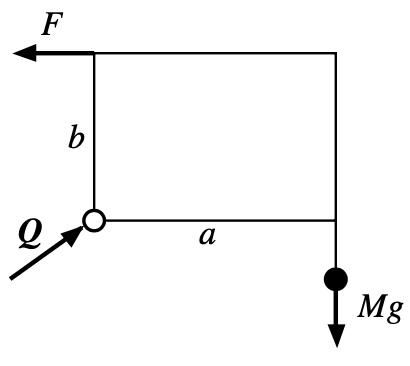
\includegraphics[width=0.22\linewidth]{../ExtFiles/rectangularLamina.png}
        \caption{The rectangular lamina.}
        \label{fig:rectangularLamina}
    \end{figure}
    \begin{itemize}
        \item The \textbf{rectangular lamina}.
        \item We're pulling on two corners, and if it's in equilibrium, the thing is not rotating. This means that
        \begin{align*}
            bF-aMg &= 0\\
            F &= \frac{a}{b}Mg
        \end{align*}
    \end{itemize}
    \item Kinetic energy.
    \begin{itemize}
        \item We have that
        \begin{equation*}
            T = \sum_\alpha\frac{1}{2}m_\alpha(\rho_\alpha\omega)^2
            = \frac{1}{2}I\omega^2
        \end{equation*}
        \item It follows that the time rate of change of the kinetic energy is
        \begin{equation*}
            \dot{T} = I\omega\dot{\omega}
            = \sum_\alpha\omega\rho_\alpha F_\phi
            = \sum_\alpha(\rho\dot{\phi})F_\phi
            = \sum_\alpha\dot{\vec{r}}_\alpha\cdot\vec{F}_\alpha
        \end{equation*}
        \item Thus, in this case, the internal forces do no work (which in some sense makes sense for a rigid body).
        \item Thus, the KE is just related to these external forces as shown above.
    \end{itemize}
    \item We'll talk about pivot points next time.
\end{itemize}




\end{document}